
\documentclass[12pt,a4paper,oneside]{article}
\usepackage[margin=1.2in]{geometry}
\usepackage{appendix}
\usepackage[dvips]{graphicx}
\usepackage{epsfig}
\usepackage{amsmath}
\usepackage{amssymb}
\usepackage{psfrag}
\usepackage[square, comma,sort,numbers]{natbib}
\usepackage{fancyhdr}
\usepackage[nottoc]{tocbibind}
\usepackage{color}
\usepackage{fixltx2e}
\usepackage{pdfpages}
\usepackage{pdflscape}
\usepackage{booktabs}
\usepackage{graphicx}
\usepackage{float}
\usepackage{afterpage}
\usepackage{subcaption}
\usepackage{lscape}
\usepackage{rotating}
\usepackage{enumitem}
\usepackage{array,tabularx}
\usepackage{fancyref}
\usepackage[dvipsnames]{xcolor}
\usepackage[colorlinks=true,allcolors=blue]{hyperref}%



\newcommand{\quotes}[1]{``#1''}

\newenvironment{conditions*}
  {\par\vspace{\abovedisplayskip}\noindent
   \tabularx{\columnwidth}{>{$}l<{$} @{\ : } >{\raggedright\arraybackslash}X}}
  {\endtabularx\par\vspace{\belowdisplayskip}}



\pagestyle{fancy}
\title{\Huge The Hat Creek Radio Observatory\\
\vspace{0.5cm}
The IF Splitter\\
\vspace{0.5cm}
\normalsize \emph{}
\vspace{3.5cm}
\begin{center}

\includegraphics[height=4cm]{titlepage/SETI_institute_logo.jpg}
\end{center}
}
\author{ 
\vspace{1cm}
\Large
\textbf{ Alexander Pollak \& Marc Jacquart} \\
SETI Institute \\ 
339 Bernardo Ave, Suite 200 \\
Mountain View, CA 94043 \\ 
Alexander.Pollak.87@gmail.com\\
}
\date{\today}



\begin{document}
\clearpage\maketitle
\thispagestyle{empty}

%\newpage
%\thispagestyle{empty}
%\section*{Abstract}
%\noindent 
%



%
%\vspace{3cm}
%\begin{flushright}
%Alexander Pollak \\ \emph{September, 2015}
%\end{flushright}

%\newpage
%\thispagestyle{empty}
%\tableofcontents
\newpage

%----------------------------------------------------------------------------------------
%	General
%----------------------------------------------------------------------------------------
%\pagestyle{plain}
\section{General}
\label{sec:General}
% ----------------------------------------------------------------

This document outlines general information regarding the IF Splitter such as the design, parts, wiring and testing. This information is aimed at detailing the entire process of creating an IF Splitter from design to manufacturing and testing. 

The purpose of the IF Splitter is to divide the incoming signal of one of the tuning (tuning "D" at the ATA) into three separate outputs. First, the signal is divided in two and one half goes directly to an output (3dB attenuation). The second output is divided in two again, leading to two more outputs with 6dB attenuation. This system allows to plug additional equipment (i.e. GNU radio, testing or monitoring devices) without unplugging the main data acquisition channel, making the ATA more polyvalent.

In this document, "IF splitter" designates the whole module while a "power splitter" designate the ZX10-2-12-S+ component that divides a signal in half. One IF splitter 6U module contains 96 power splitter components.
%----------------------------------------------------------------------------------------
%	CAD Design and Drawings
%--------------------------------------------------------------------------------------

\section{CAD Design and Drawings}
\label{sec:CAD}
% ----------------------------------------------------------------
This section includes a description of the CAD design. Figure \ref{fig:CAD_outside} shows the outside of the IF splitter module with the front panel containing the two groups of 6dB outputs. Figure \ref{fig:CAD_inside} shows the IF splitter module open, with the mounts and signal splitter components but no cable. The left CAD drawing shows the back panel with the group of inputs on top and the group of 3dB Outputs below. Both the front and back panel look similar in the number and placement of the SMA connectors. As a visual reference, it can be noted that the two handles are on the front of the IF Splitter. The part list is available in appendix \ref{sec:Part_List}. The Drawings are available in appendix \ref{sec:Drawings}.

\hfill \break

%
\begin{figure}[H]
\centering
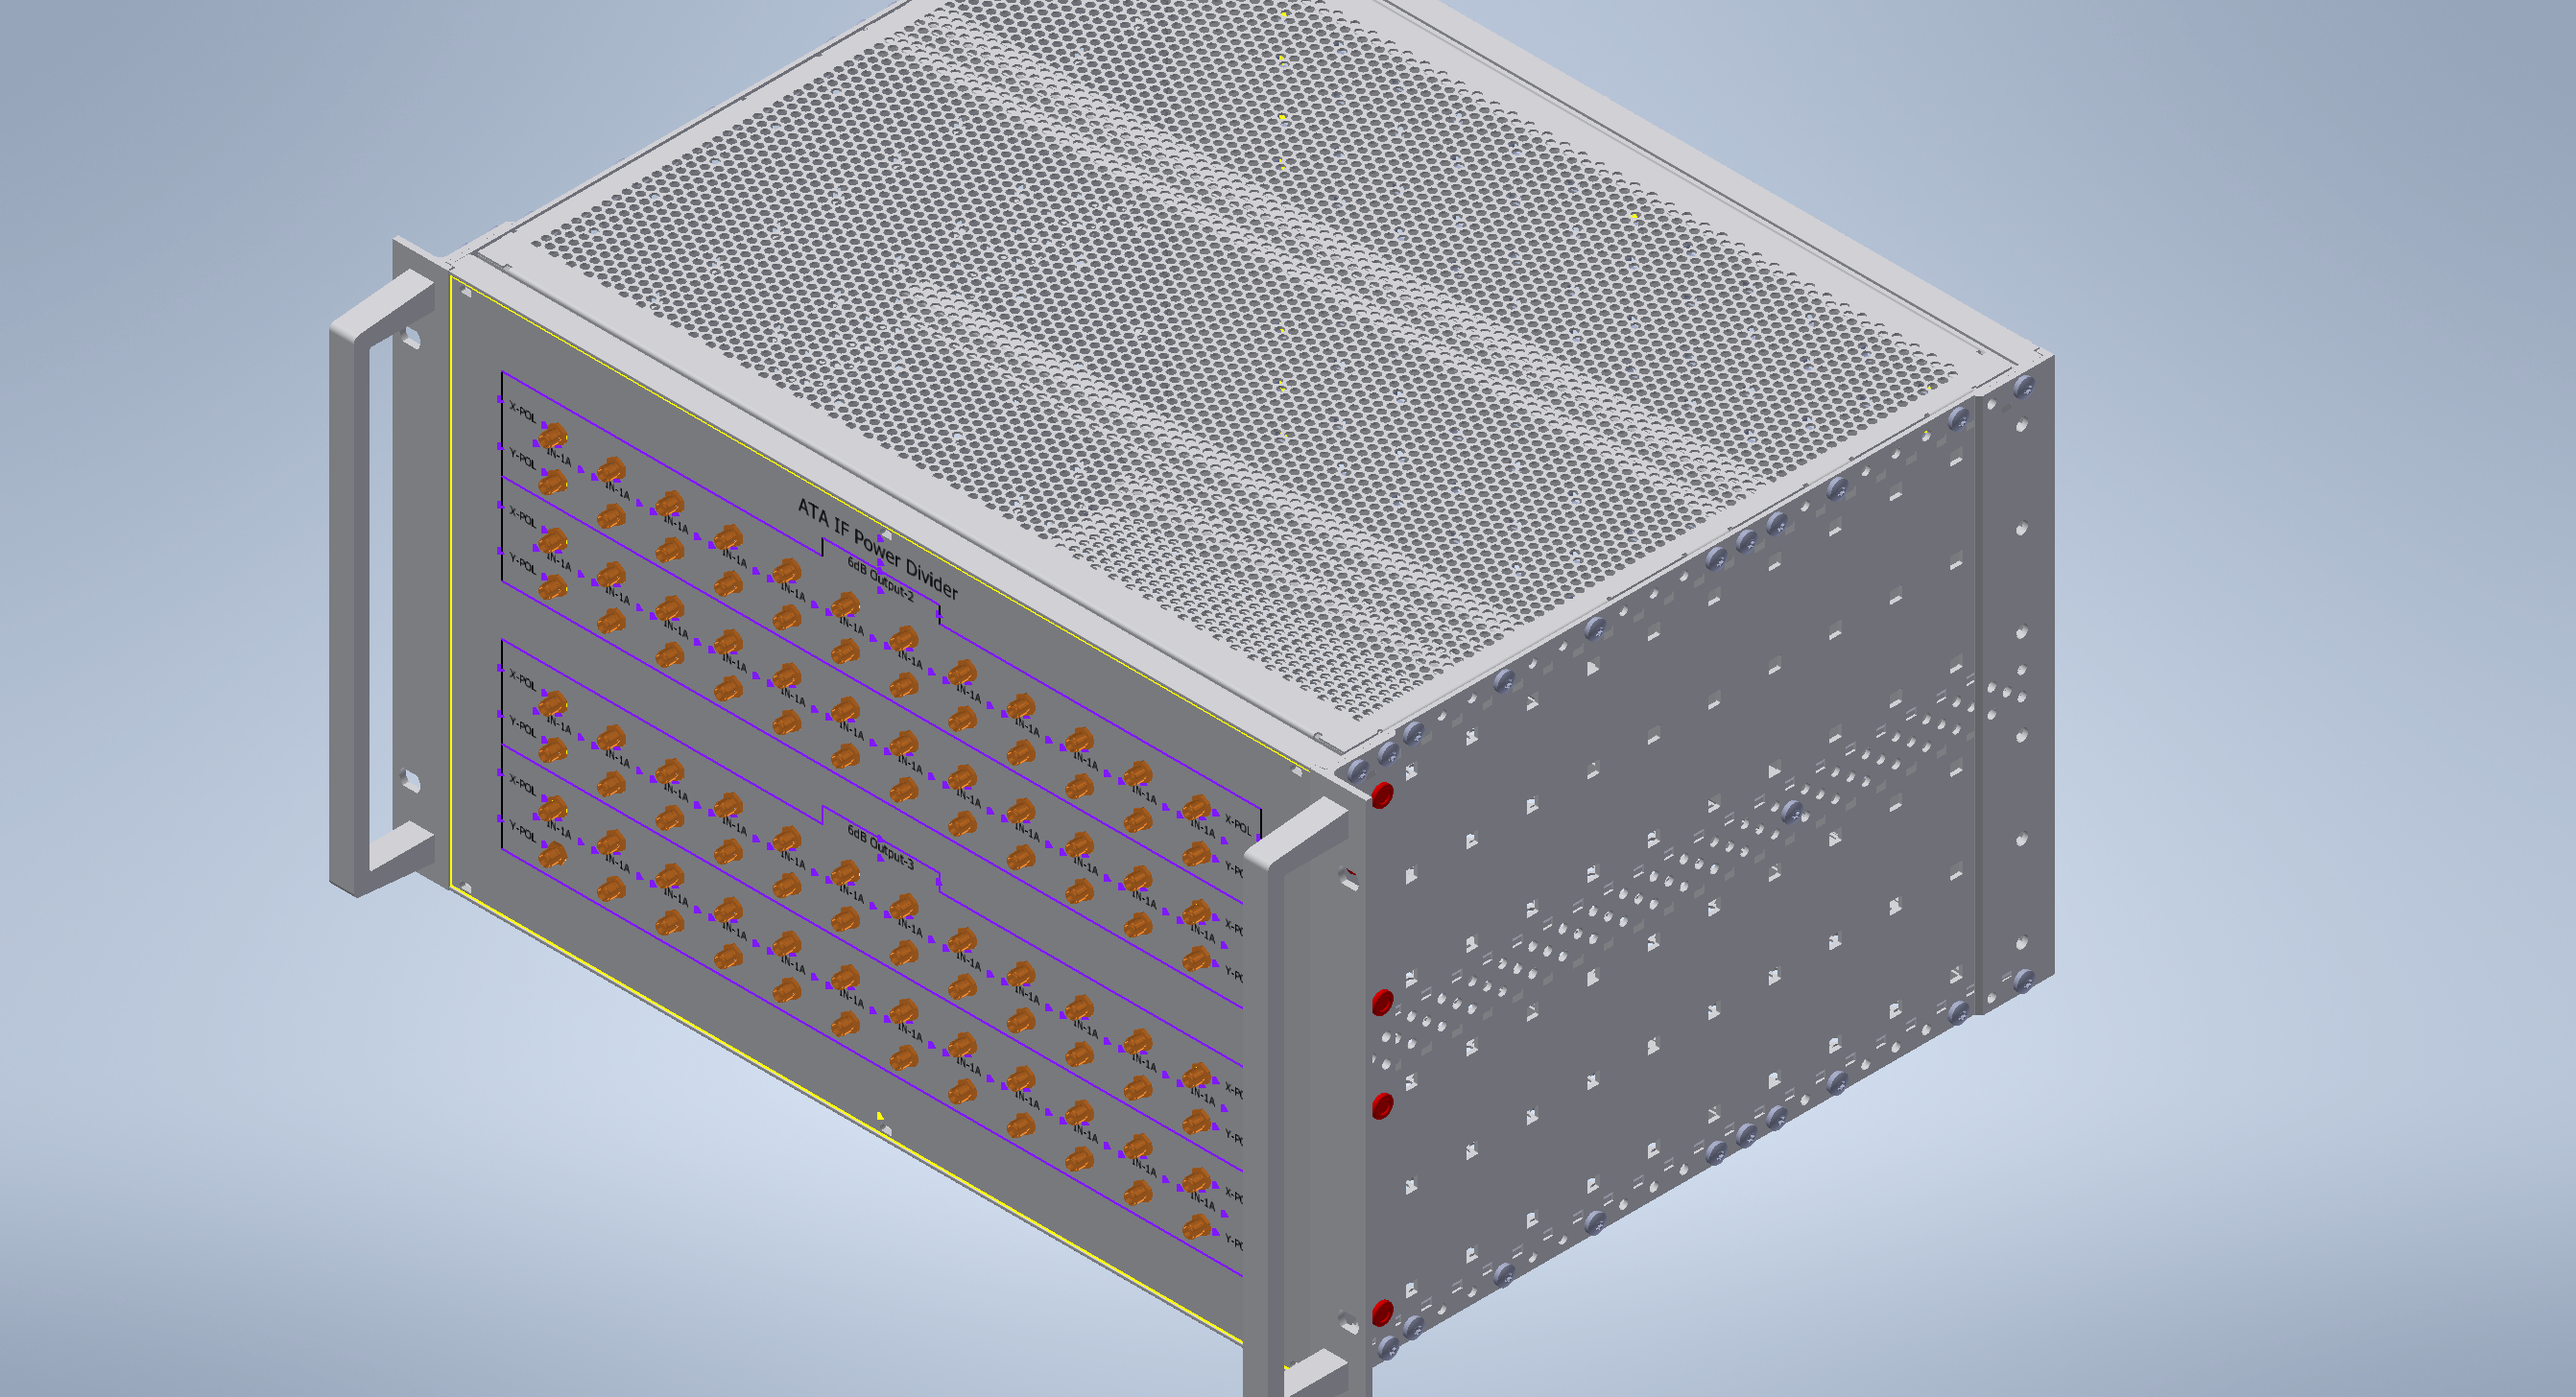
\includegraphics[width=1\linewidth]{figures/CAD_outside.png}
\caption{Outside CAD view of the IF splitter.}
\label{fig:CAD_outside}
\end{figure}
%

%
\begin{figure}[H]
\centering
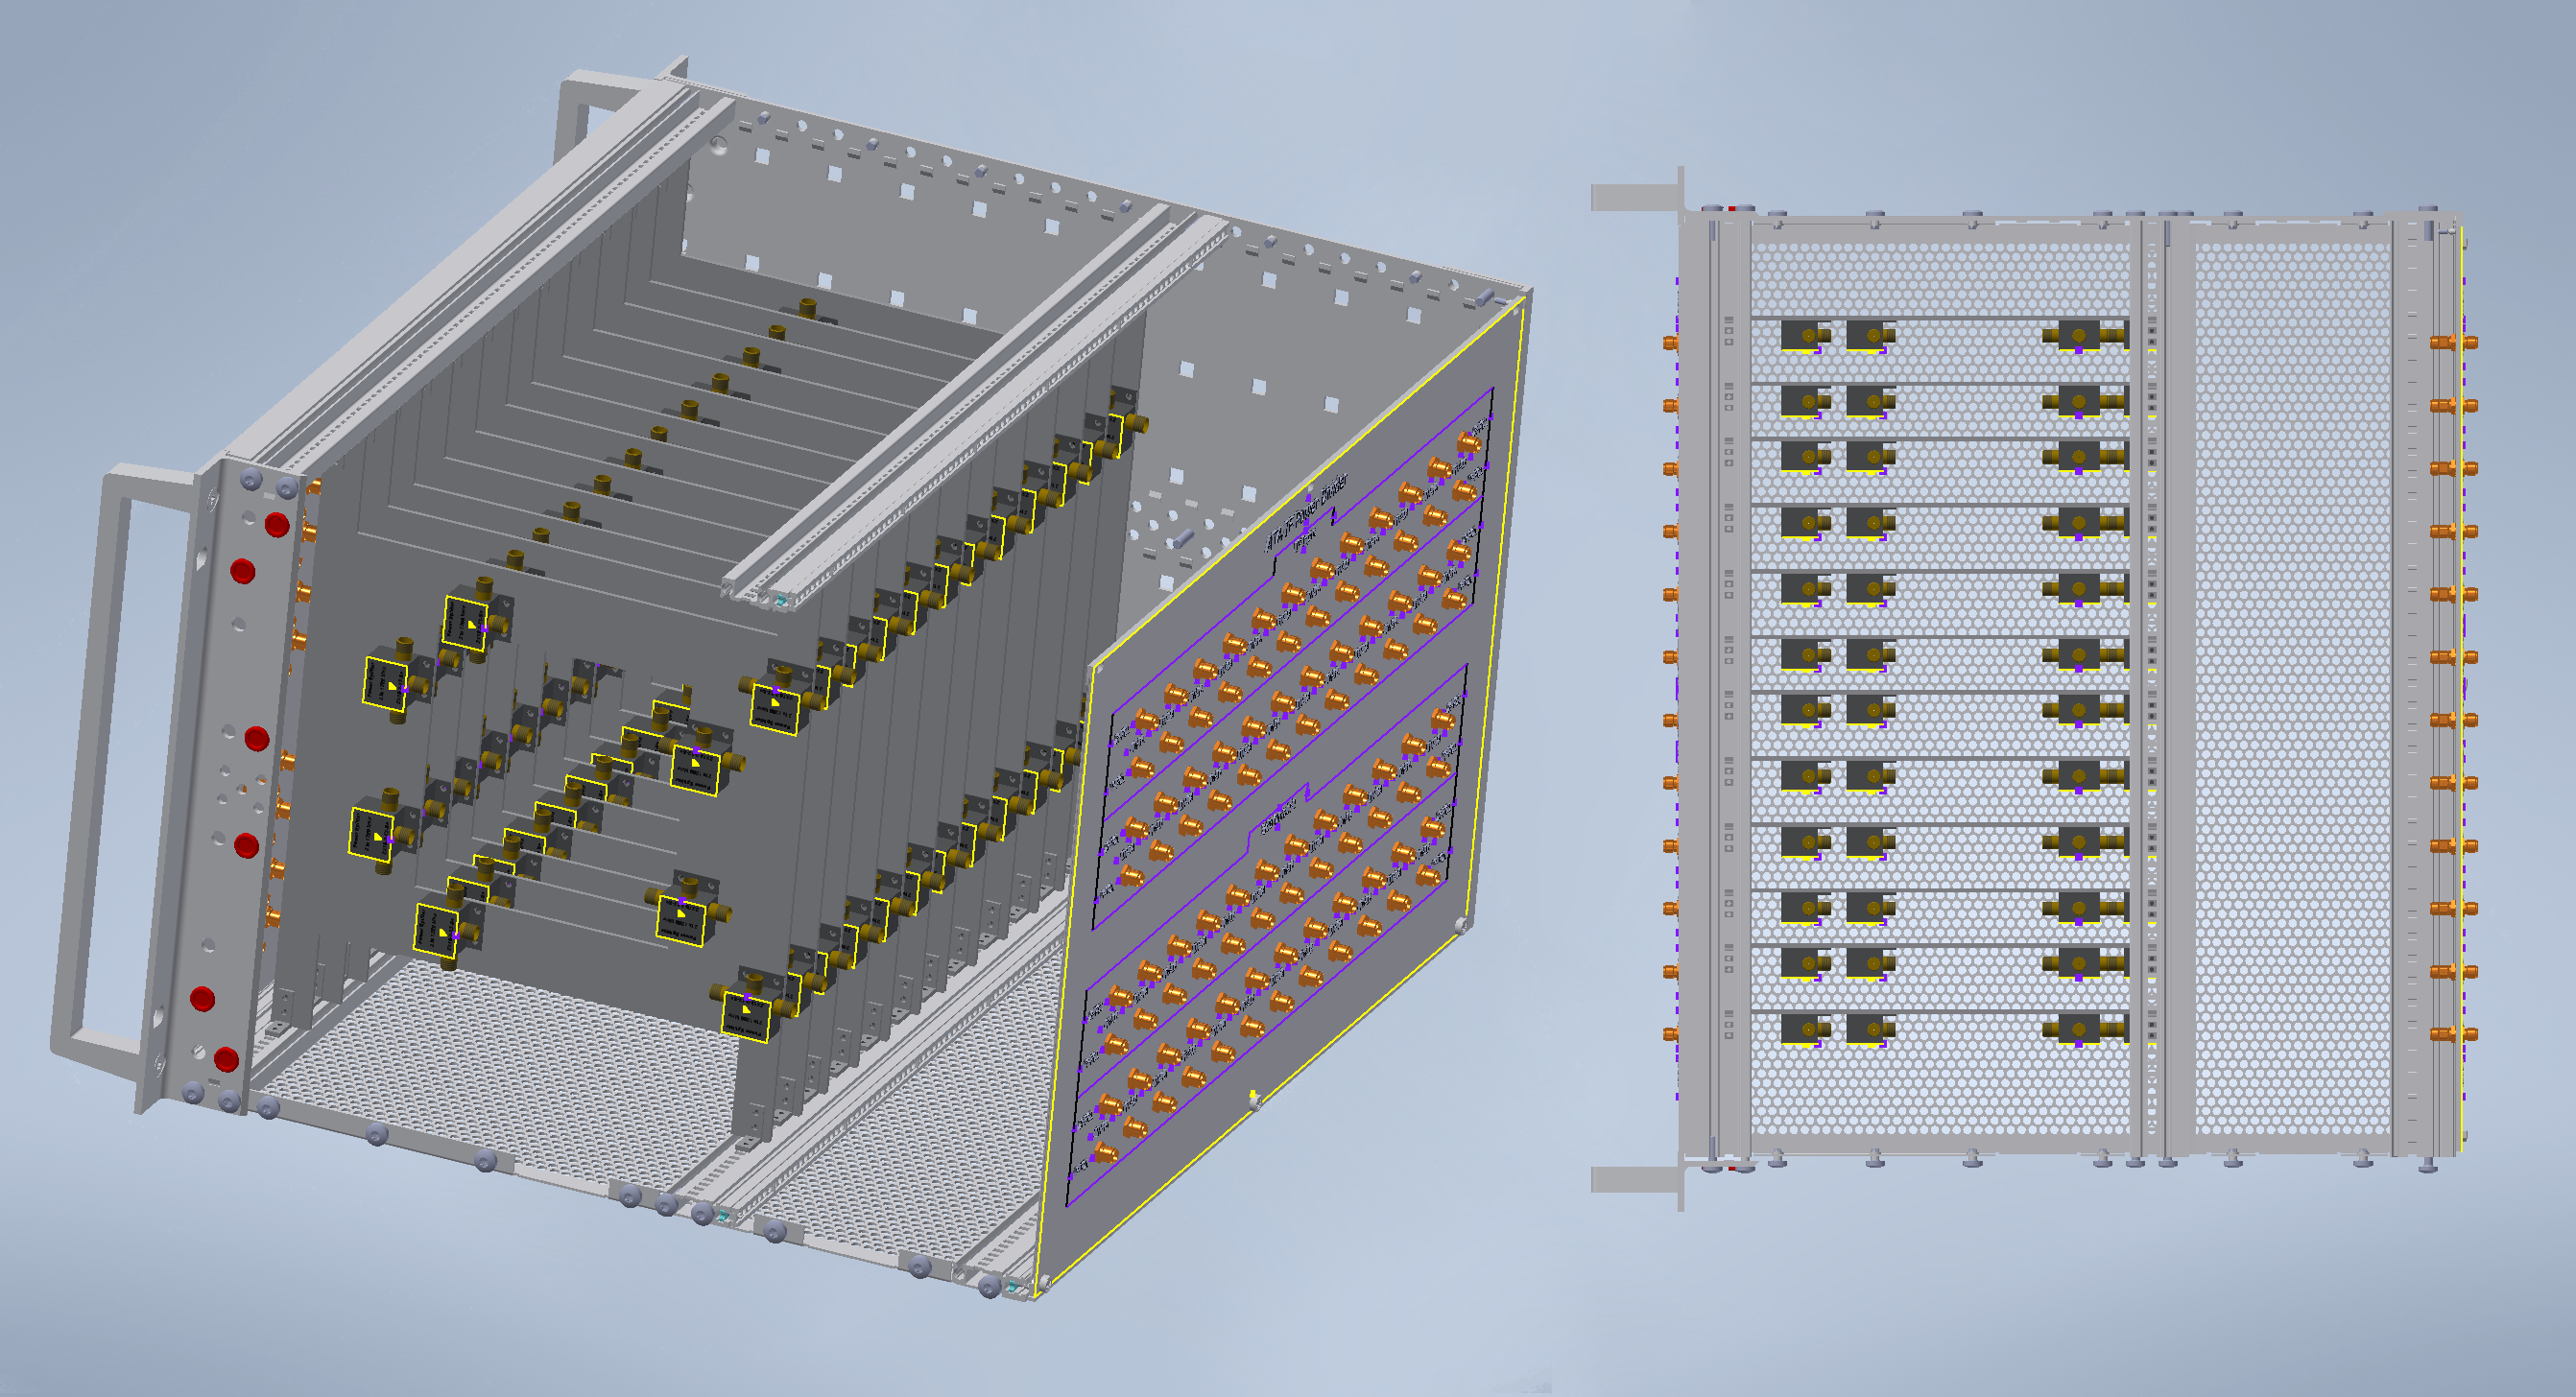
\includegraphics[width=1\linewidth]{figures/CAD_inside.png}
\caption{Left shows a three-dimensional CAD view of the inside of the IF splitter. Right shows the same, but from a top view. The cables are not represented on both images for more clarity.}
\label{fig:CAD_inside}
\end{figure}
%

\newpage
\subsection{Design}
\label{sec:Design}
% ----------------------------------------------------------------
The front and back panels each contain two groups of 12$\times$4 SMA connectors. On the back panel, the top group is for the "IF Input" and the bottom for the "3dB Output-1". The front panel contains the two groups of "6dB Output-2" and "6dB Output-3". The front and back panel design are available in appendix \ref{sec:Drawings}. A schematic of the IF Splitter for one input is shown in figure \ref{fig:IF_Splitter_Diagram}. Two inputs are used per antenna for the X and Y polarization signals. Each module contains 48 input connections, which allow to split the signal of 24 antennas. Thus two IF splitter modules are installed for the 42 ATA antennas, leaving 6 input pairs unused for spares.

All the components in the IF splitter are passive so the module doesn't require any power supply.

%
\begin{figure}[H]
\centering
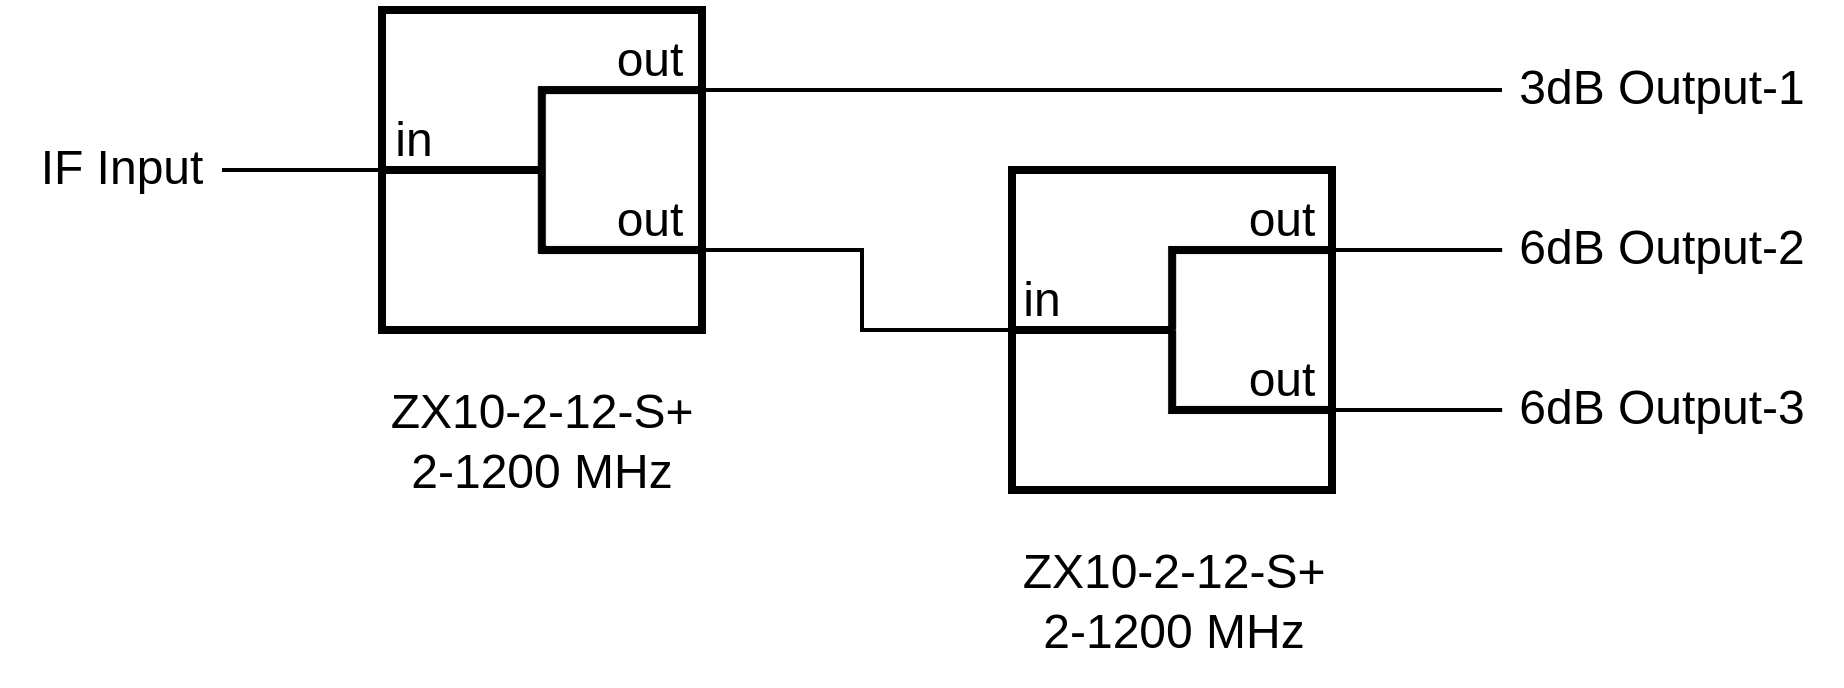
\includegraphics[width=1\linewidth]{schematics/IF_splitter.drawio.png}
\caption{Signal splitter diagram for one input, repeated 48 times in the IF Splitter.}
\label{fig:IF_Splitter_Diagram}
\end{figure}
%

%--
\subsection{Wiring}
\label{sec:Wiring}
% ----------------------------------------------------------------
The Mini-Circuits power splitter components are screwed on 12 separate mounts. The wiring schematic of one mount is shown in figure \ref{fig:splitter_full_draw} and a picture of the complete circuit in figure \ref{fig:splitter_wiring}.

%
\begin{figure}[H]
\centering
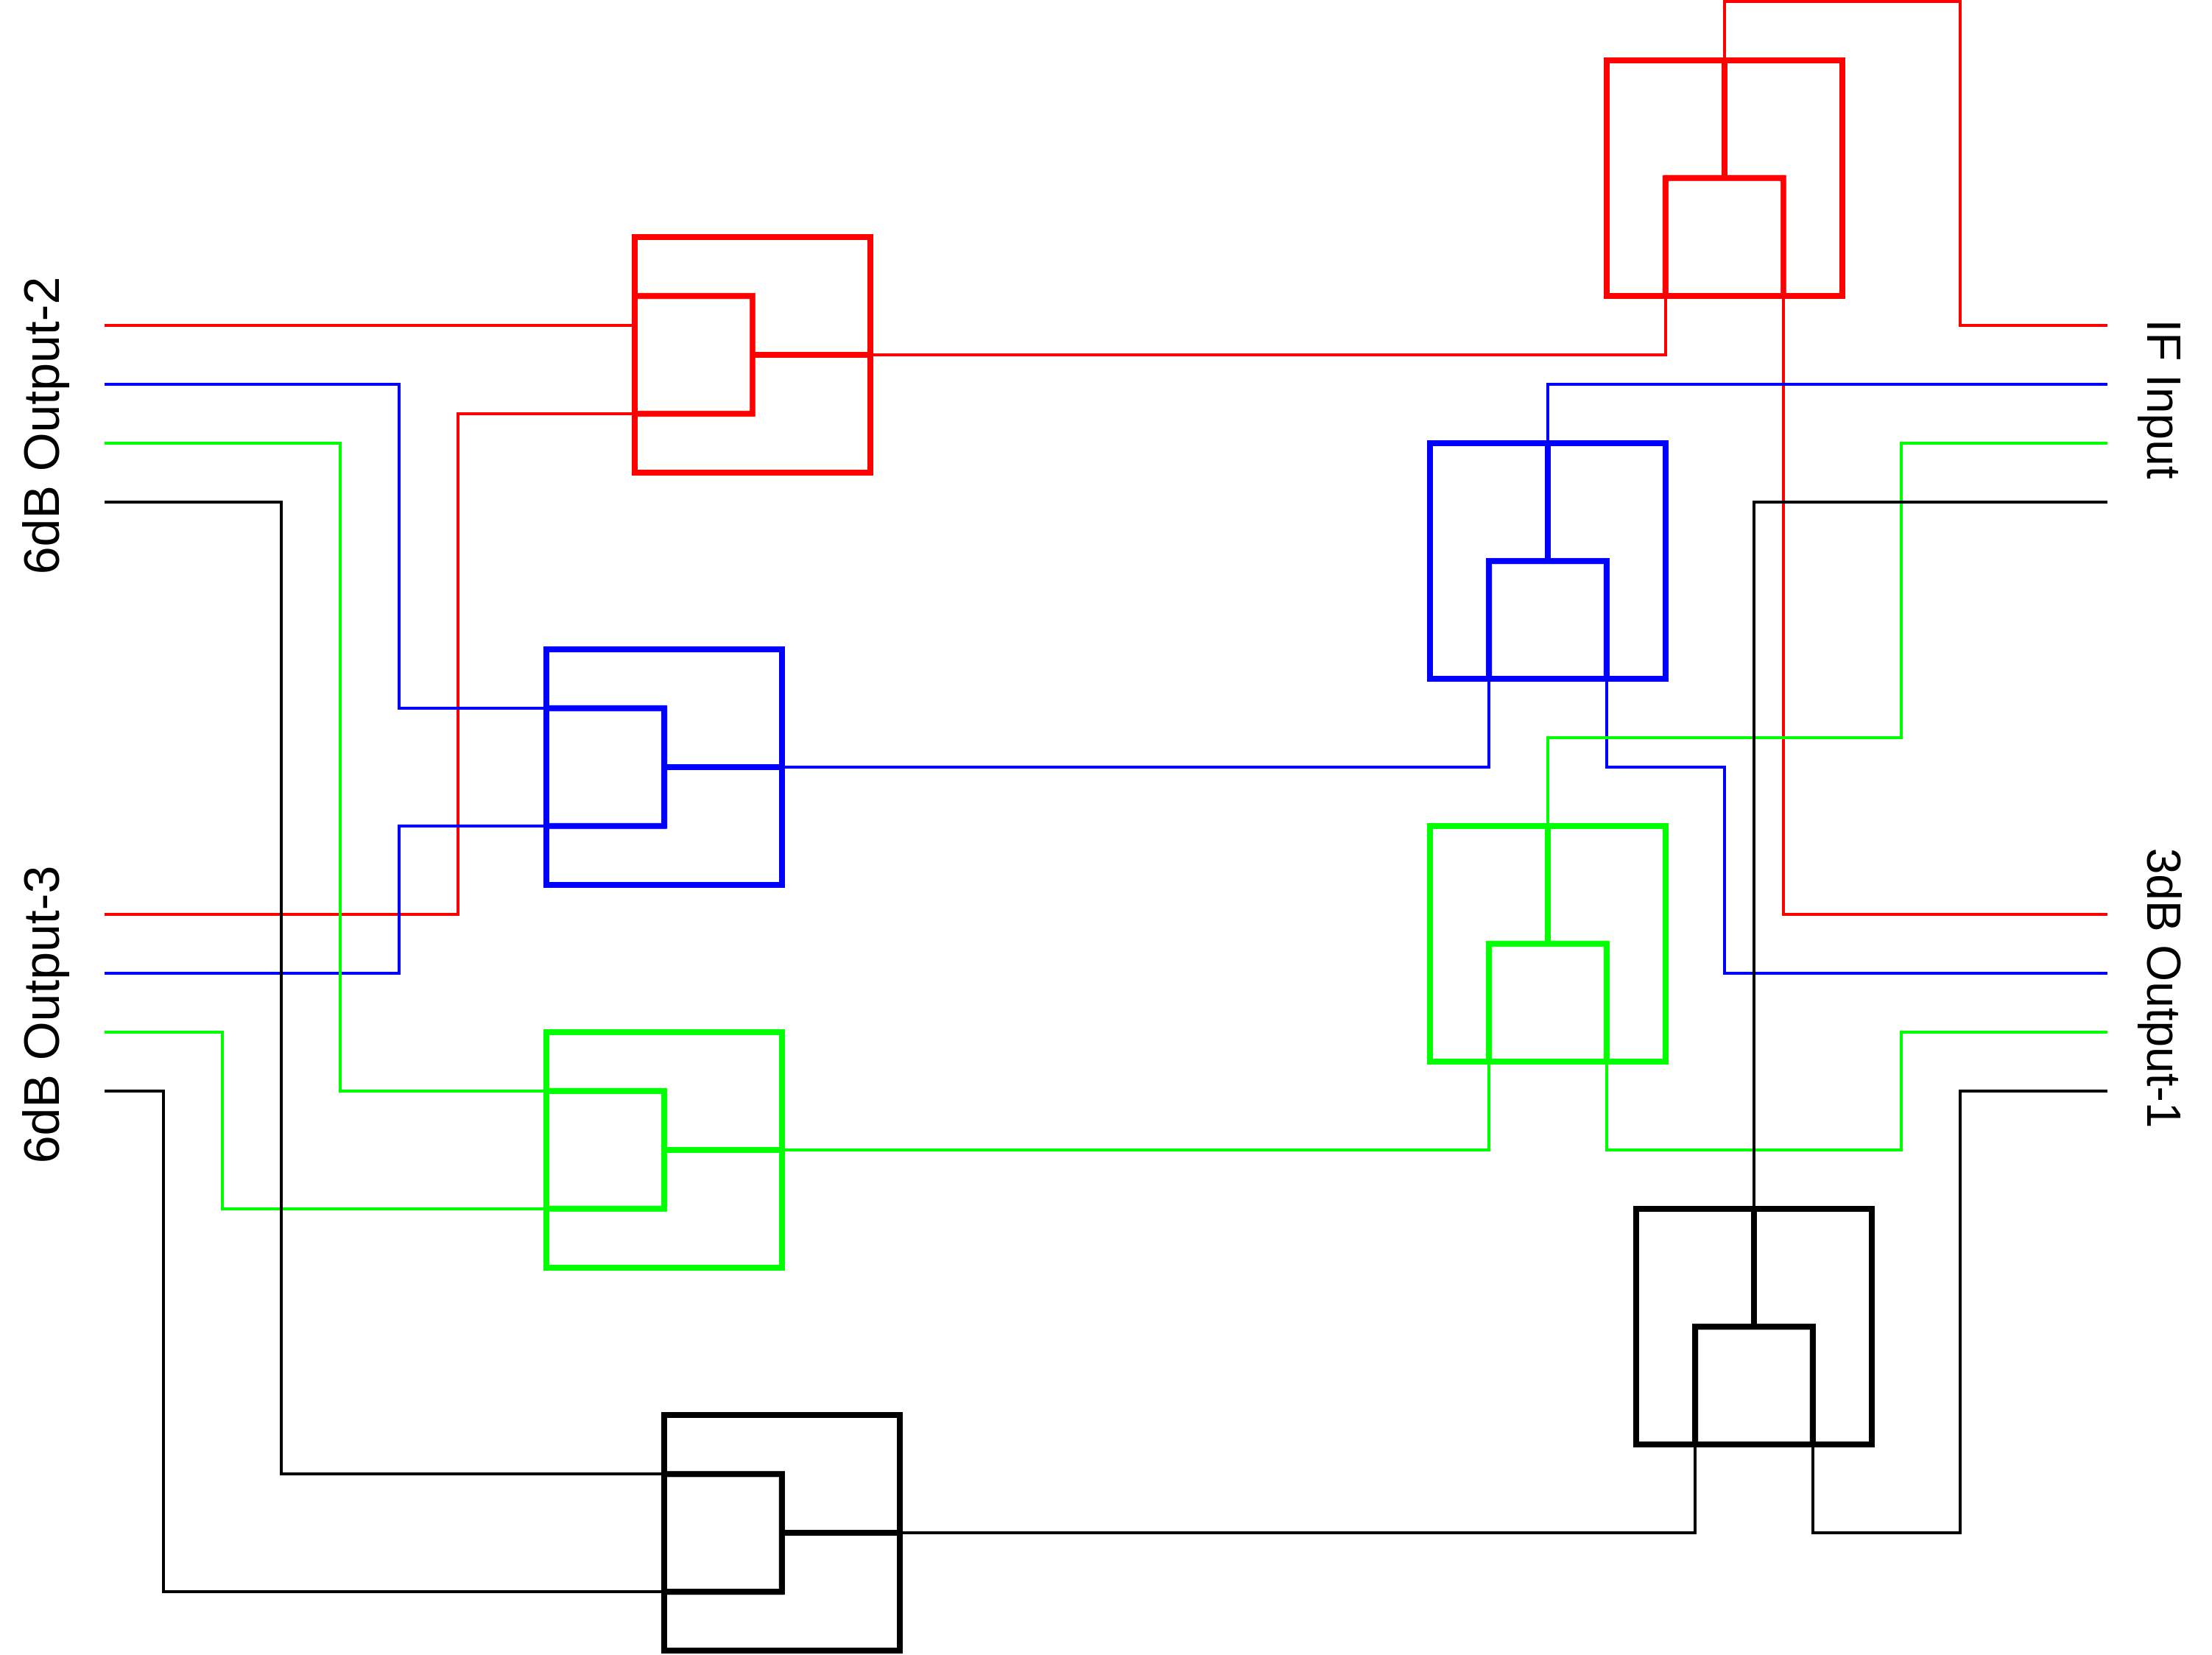
\includegraphics[width=0.9\linewidth]{schematics/IF_splitter_full_mount.drawio.png}
\caption{Wiring diagram for one mount.}
\label{fig:splitter_full_draw}
\end{figure}
%

%
\begin{figure}[H]
\centering
\includegraphics[width=0.9\linewidth]{figures/IFSplitter_wiring.png}
\caption{Picture of one completed mount able to split four input signals.}
\label{fig:splitter_wiring}
\end{figure}
%



\section{Testing}
\label{sec:Testing}


\subsection{Setup}
\label{sec:Testing_Setup}
% ----------------------------------------------------------------
The Vector Network Analyzer (VNA) is used to make a measurement of the scattering matrix. The pre-made "IFSplitter" measurement setup configuration can be selected on the HCRO VNA (Model: Agilient Technologies N5230C) to get the relevant scale and information for the plots. Two 1-meter probe cables "ABC-CA18-SMSM-1.OM" are used. A special wrench that delivers only 0.9$\thinspace$N$\cdot$m or 8$\thinspace$in$\cdot$lbs of torque must be used to tighten all the SMA connectors in place. 


The first step is to calibrate the VNA using the open-short-load calibration kit. In our case, we are not able to calibrate the VNA, hence we use the math function to normalize the $S_{12}$ and $S_{21}$ transmission loss to $0\thinspace$dB over the required frequency range.To do so, both probes are shorted wit a 1.2$\thinspace$cm female-female SMA connector, as shown in figure \ref{fig:VNA_Normalize_Setup}. Then select the scattering matrix plot elements $S_{12}$, $S_{21}$ and select on the VNA: Memory$\rightarrow$Normalize. The result should be $S_{12}=0\thinspace$dB and $S_{21}=0\thinspace$dB for all frequencies on the VNA plots, as shown in figure \ref{fig:VNA_normalized}.

%
\begin{figure}[H]
\centering
\includegraphics[width=1\linewidth]{figures/VNA_Normalize_Setup.png}
\caption{VNA setup for $S_{12}$ and $S_{21}$ normalization.}
\label{fig:VNA_Normalize_Setup}
\end{figure}
%
%
\begin{figure}[H]
\centering
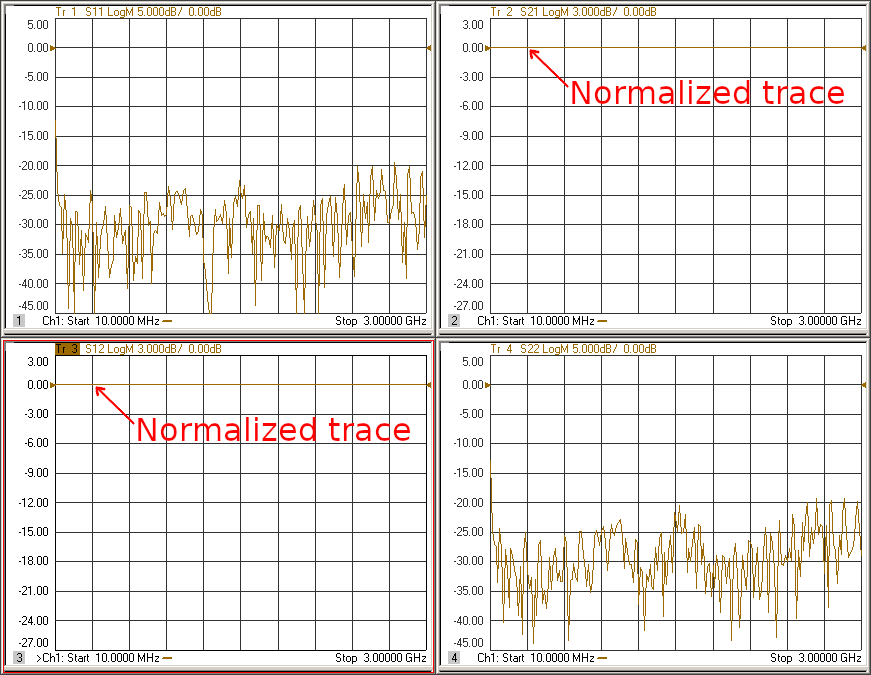
\includegraphics[width=0.9\linewidth]{figures/Normalized.png}
\caption{Scattering matrix after $S_{12}$ and $S_{21}$ normalization.}
\label{fig:VNA_normalized}
\end{figure}
%

\subsection{Method \& Desired Results}
\label{sec:Testing_Method}
% ----------------------------------------------------------------

The VNA port 1 is connected to the "IF Input" while the VNA port 2 is connected in turn to "3dB Output-1", "6dB Output-2" and "3dB Output-3".Two 18$\thinspace$GHz 50$\thinspace\Omega$ terminators are used for the pair of SMA output connectors that are not connected to the VNA. Each measurement is individually recorded as a screenshot of the four S-parameters. These steps have to be reproduced 48 times for all the channels of the IF Splitter module.

An example of the expected measurement of "3dB Output-1" is shown in figure \ref{fig:VNA_3dB-1}. At 10$\thinspace$MHz, $S_{12}$ and $S_{21}$ are slightly below -3dB because of loss. The loss increases significantly after 1.8$\thinspace$GHz, which is above the rated value of 1.2$\thinspace$GHz from the "ZX10-2-12-S+" power splitter. The return loss ($S_{11}$ and $S_{22}$) must be below $-20\thinspace$dB.

The result of for both "6dB Output-2" and "6dB Output-3" must be similar to each-other, the difference being only the output of the second power splitter module. An example is given respectively in figure \ref{fig:VNA_6dB-2} and \ref{fig:VNA_6dB-3}. Here again an increasing loss is observed with the frequency, that accelerate after 1.8$\thinspace$GHz. Also here again the return loss must be below $-20\thinspace$dB.
%
\begin{figure}[]
\centering
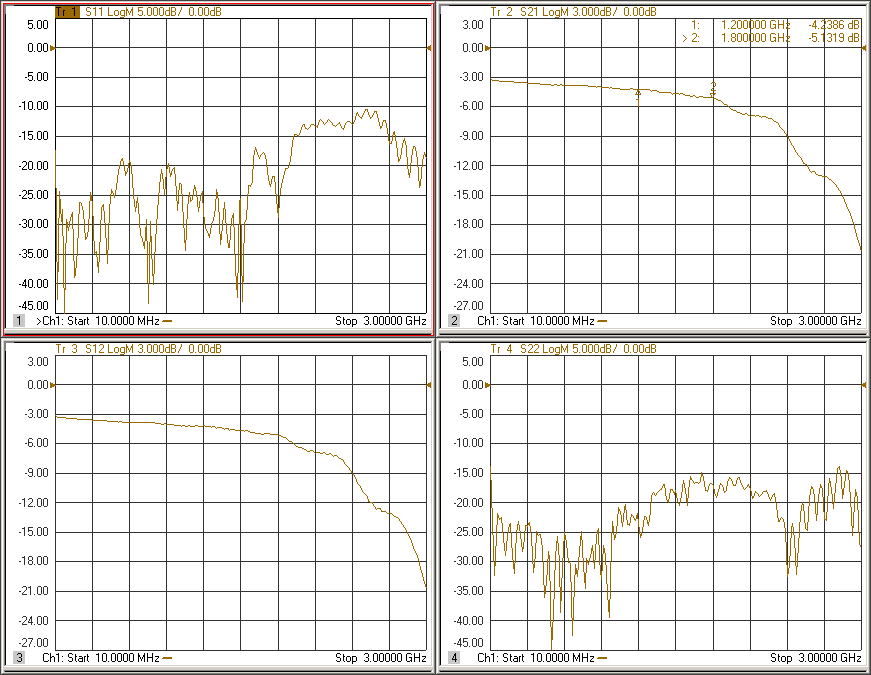
\includegraphics[width=0.9\linewidth]{figures/3dB-1.png}
\caption{Scattering matrix for "3dB Output-1".}
\label{fig:VNA_3dB-1}
\end{figure}
%
%
\begin{figure}[H]
\centering
\includegraphics[width=0.9\linewidth]{figures/6dB-2.png}
\caption{Scattering matrix for "6dB Output-2".}
\label{fig:VNA_6dB-2}
\end{figure}
%
%
\begin{figure}[H]
\centering
\includegraphics[width=0.9\linewidth]{figures/6dB-3.png}
\caption{Scattering matrix for "6dB Output-3".}
\label{fig:VNA_6dB-3}
\end{figure}
%

\subsection{Module verification}
\label{sec:Testing_Troubleshooting}
% ----------------------------------------------------------------
Each signal path must be measured with the VNA and documented via a measurement result screenshot. If the result doesn't look like the example figures \ref{fig:VNA_3dB-1} to \ref{fig:VNA_6dB-3}, look at the different output measurement for a same input to try to locate the problem with the schematic in figure \ref{fig:IF_Splitter_Diagram}. If there is no transmission, verify that the circuit corresponds to the schematic in figure \ref{fig:splitter_full_draw}. 

If the transmission signal curves of $S_{12}$ and $S_{21}$ aren't smooth (figures \ref{fig:VNA_3dB-1} to \ref{fig:VNA_6dB-3} show how they should look), there must be a bad connection along the signal path. First verify that the probes and terminators are attached correctly on the front panel with the right amount of torque. Then have a visual inspection of the mount and connection to verify that no component is damaged or not mounted properly. If everything looks good, it can either be a bad cable connection or a bad power splitter. If all the cables are connected and torqued properly, verify the power splitter modules themselves by plugging the VNA to their output directly. The unused third connector must be terminated. Finally, if the problem is still there, test the cables themselves using the VNA.
\newpage
 
%----------------------------------------------------------------------------------------
%	Appendix: Attemplifier Module Enclosure Drawings
%----------------------------------------------------------------------------------------

\appendix
% ----------------------------------------------------------------

% To include pages from other PDFs
% 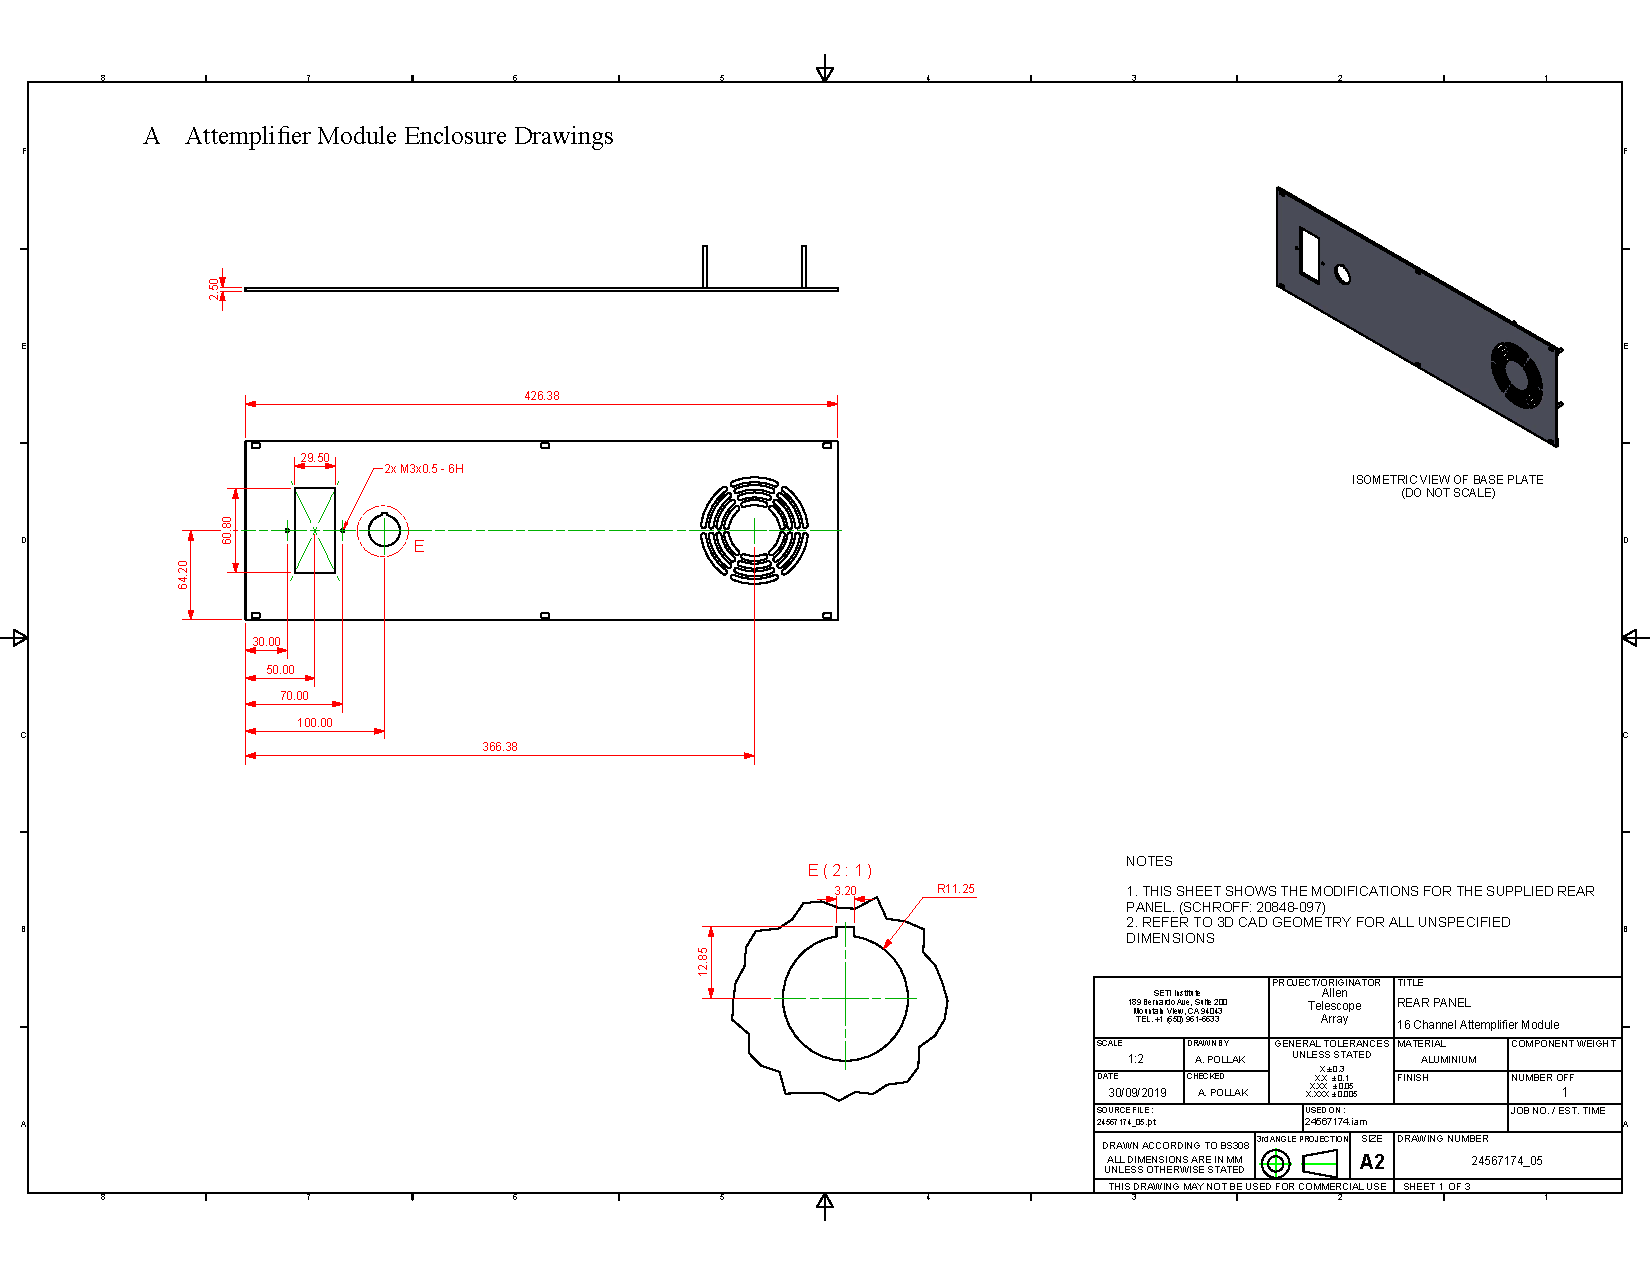
\includepdf[pages=-, landscape=true]{Documentation/PDFs/24567174_05(copy).pdf}


%----------------------------------------------------------------------------------------
%	Appendix: IF splitter Component List
%----------------------------------------------------------------------------------------
\begin{landscape}
\section{Component List of the IF Splitter}\label{sec:Part_List}

% ----------------------------------------------------------------

\begin{table}[H]
\centering
\resizebox{1.5\textwidth}{!}{%
\begin{tabular}{@{}lllllll@{}}
\toprule
Qty & Unit & Description & Manufacturer & PN Manufacturer & Distributor & PN Distributor\\
\midrule
1 & Each & 6U EuropacPRO kit, heavy design, shielded, without front handles & Schroff & 24563-474 & Distrelec & 110-28-346 \\
1 & Each & Front Panel & Front Panel Express, LLC & ATA-IFD-AP-24567274\_100F.fpd &&\\
1 & Each & Rear panel & Front Panel Express, LLC & ATA-IFD-AP-24567274\_100R.fpd &&\\
12 & Each & Mounting Panel & Front Panel Express, LLC & ATA-IFD-AP-24567274\_200.fpd &&\\
48 & Each & Mounting Bracket & Front Panel Express, LLC & ATA-IFD-AP-24567274\_201.fpd &&\\
96 & Each & 2 Ways Power Splitter, 2 - 1200 MHz, 50$\Omega$ & MiniCircuit & ZX10-2-12-S+ &&\\
%
4 & Pack & Machine Screw, M2.5, 5mm & TR FASTENINGS & 173-202579H & Newark & 25M0782\\
% 1 pach is 100 screw and we need 336:
% 12 * 12 = 144 for L-brackets
% 16 * 12 = 192 to attach power splitter modules on mount
%

48 & Each & 5 Inch SMA coaxial cable & Atlantic Microwave & ASF1-005-520003-S4S4 &&\\
96 & Each & 6 Inch SMA Male to SMA Female Bulkhead cable & Pasternack & PE39433-6 &&\\
96 & Each & 12 Inch SMA Male to SMA Female Bulkhead cable & Pasternack & PE39433-12 &&\\
\bottomrule            
\end{tabular}}
\label{tab:IF_components}
\end{table}

%----------------------------------------------------------------------------------------
%	Appendix: Control Board Schematics
%----------------------------------------------------------------------------------------

\section{Drawings}
\label{sec:Drawings}
Below are the drawings of the back panel, Power Splitter Mount and L-shape attachment brackets.
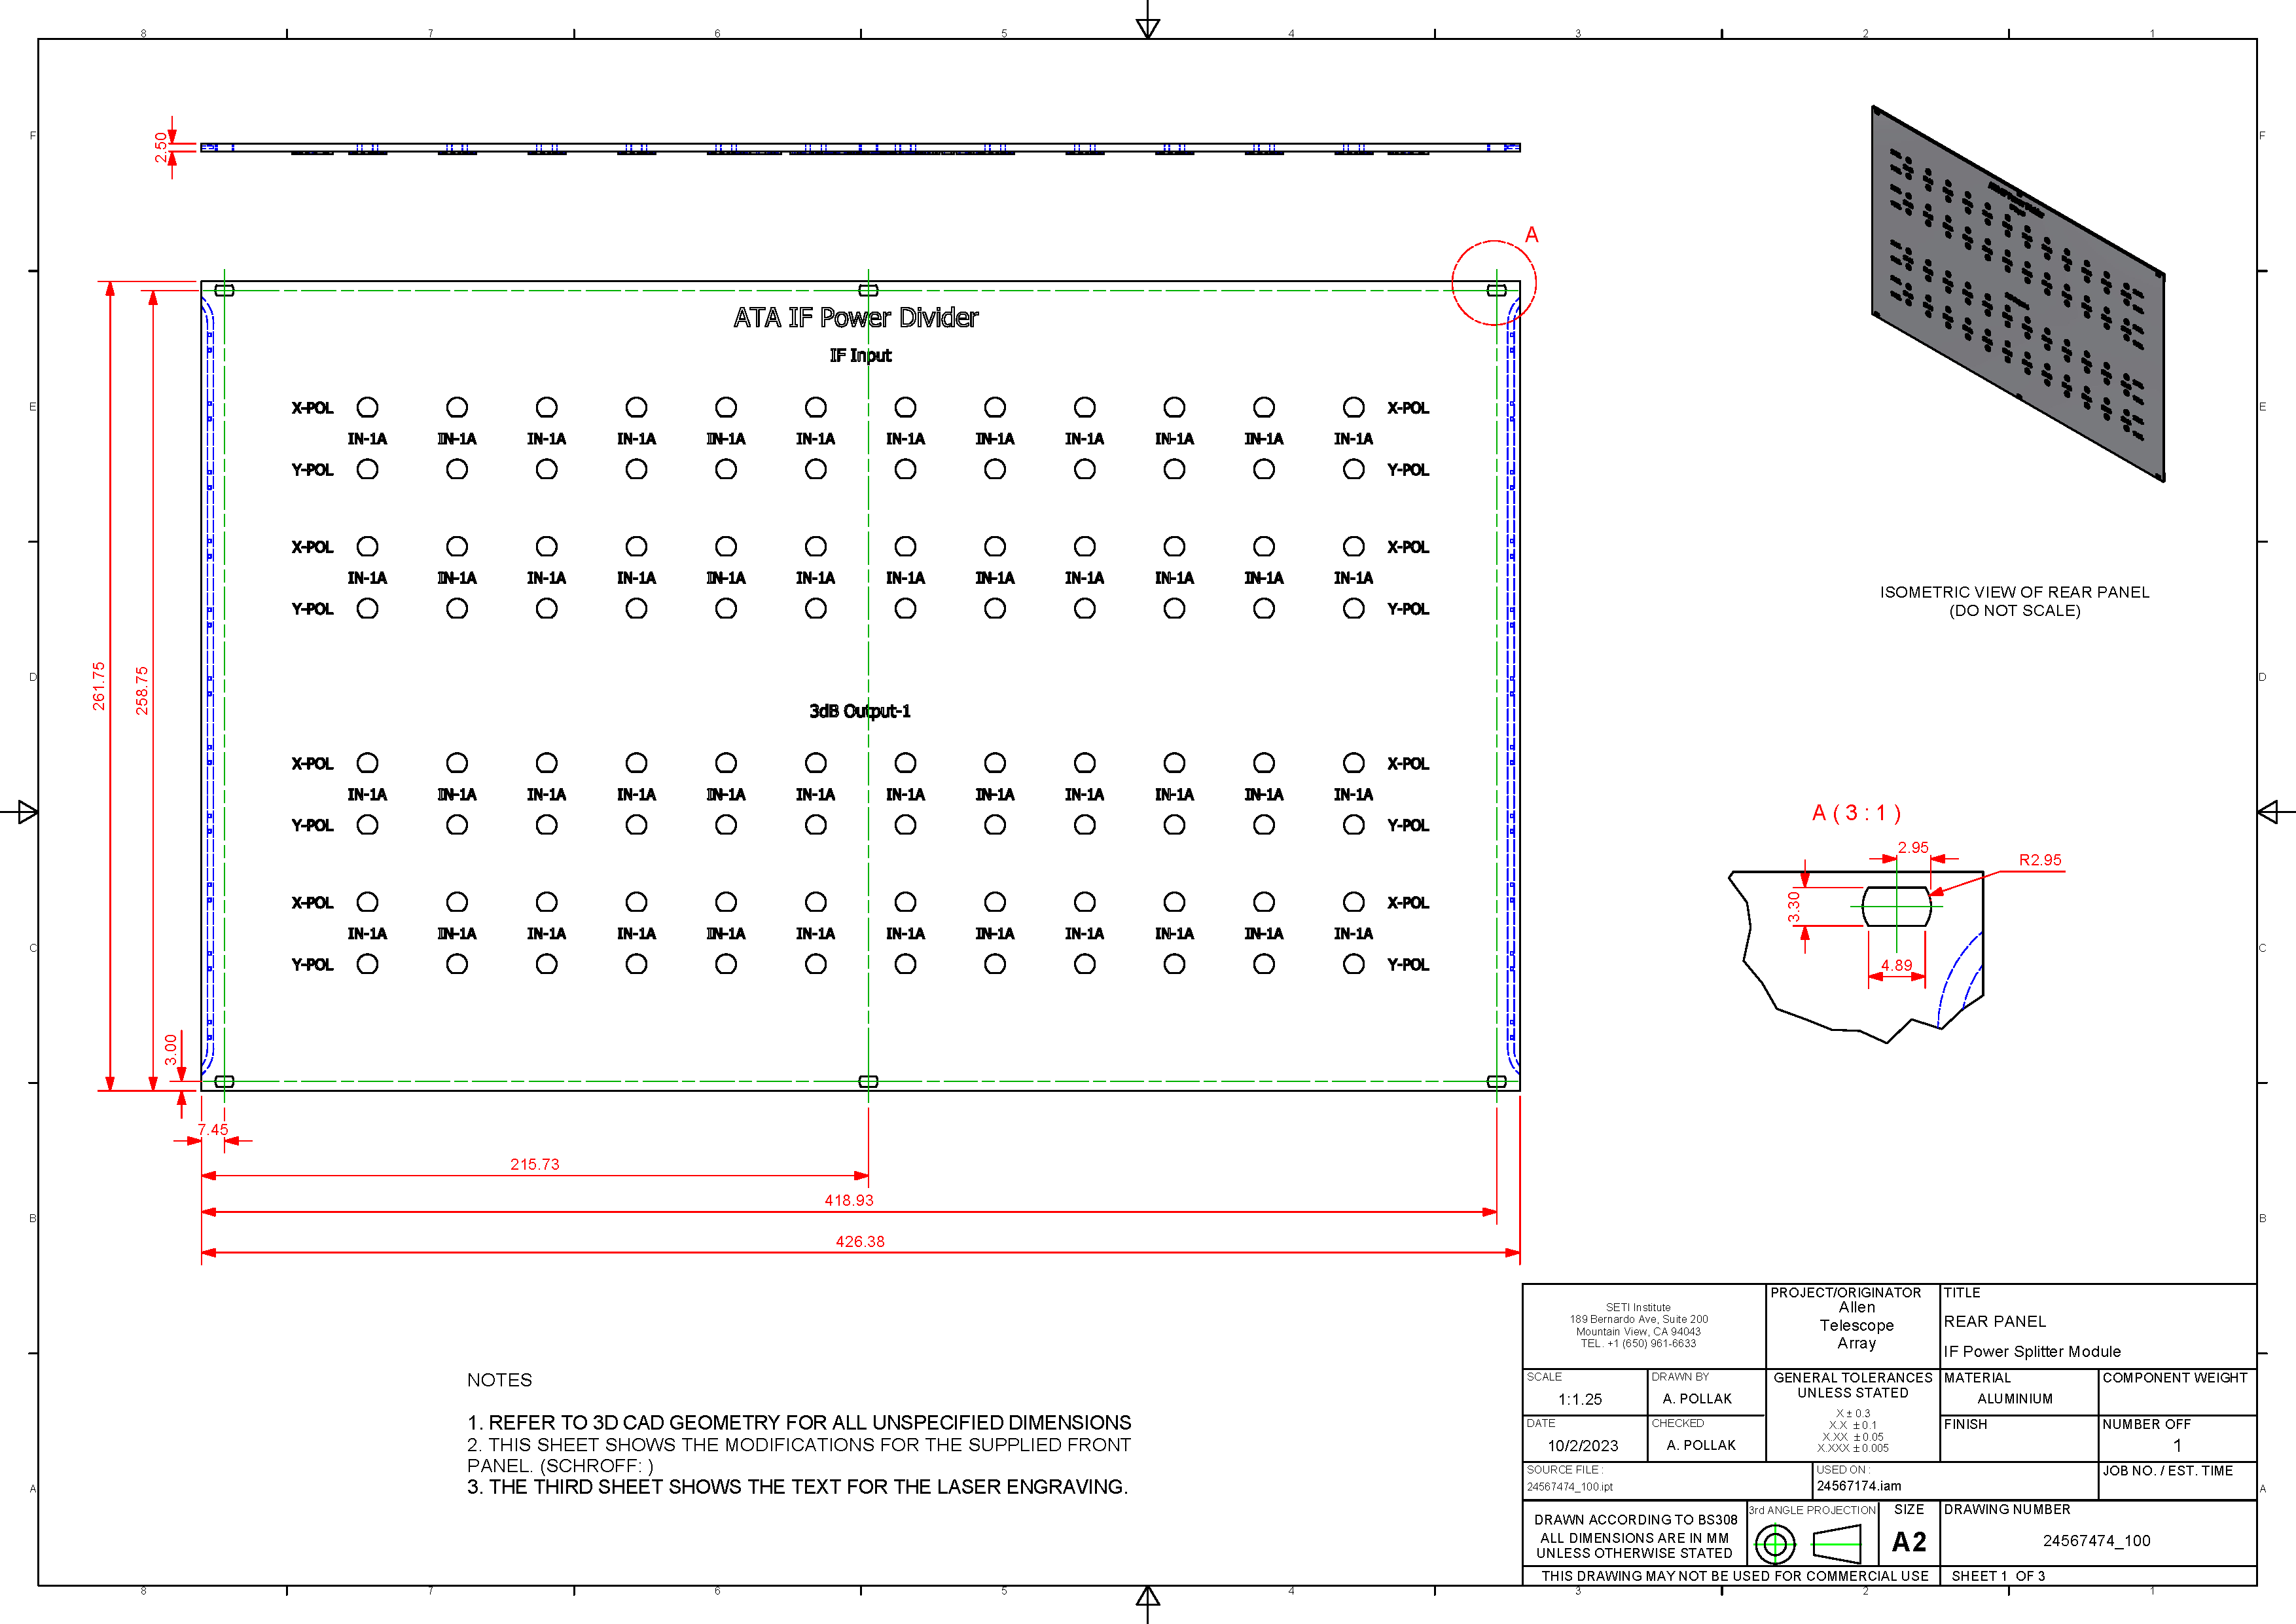
\includepdf[pages=1-2, landscape=true]{PDFs/24567474_100.pdf}
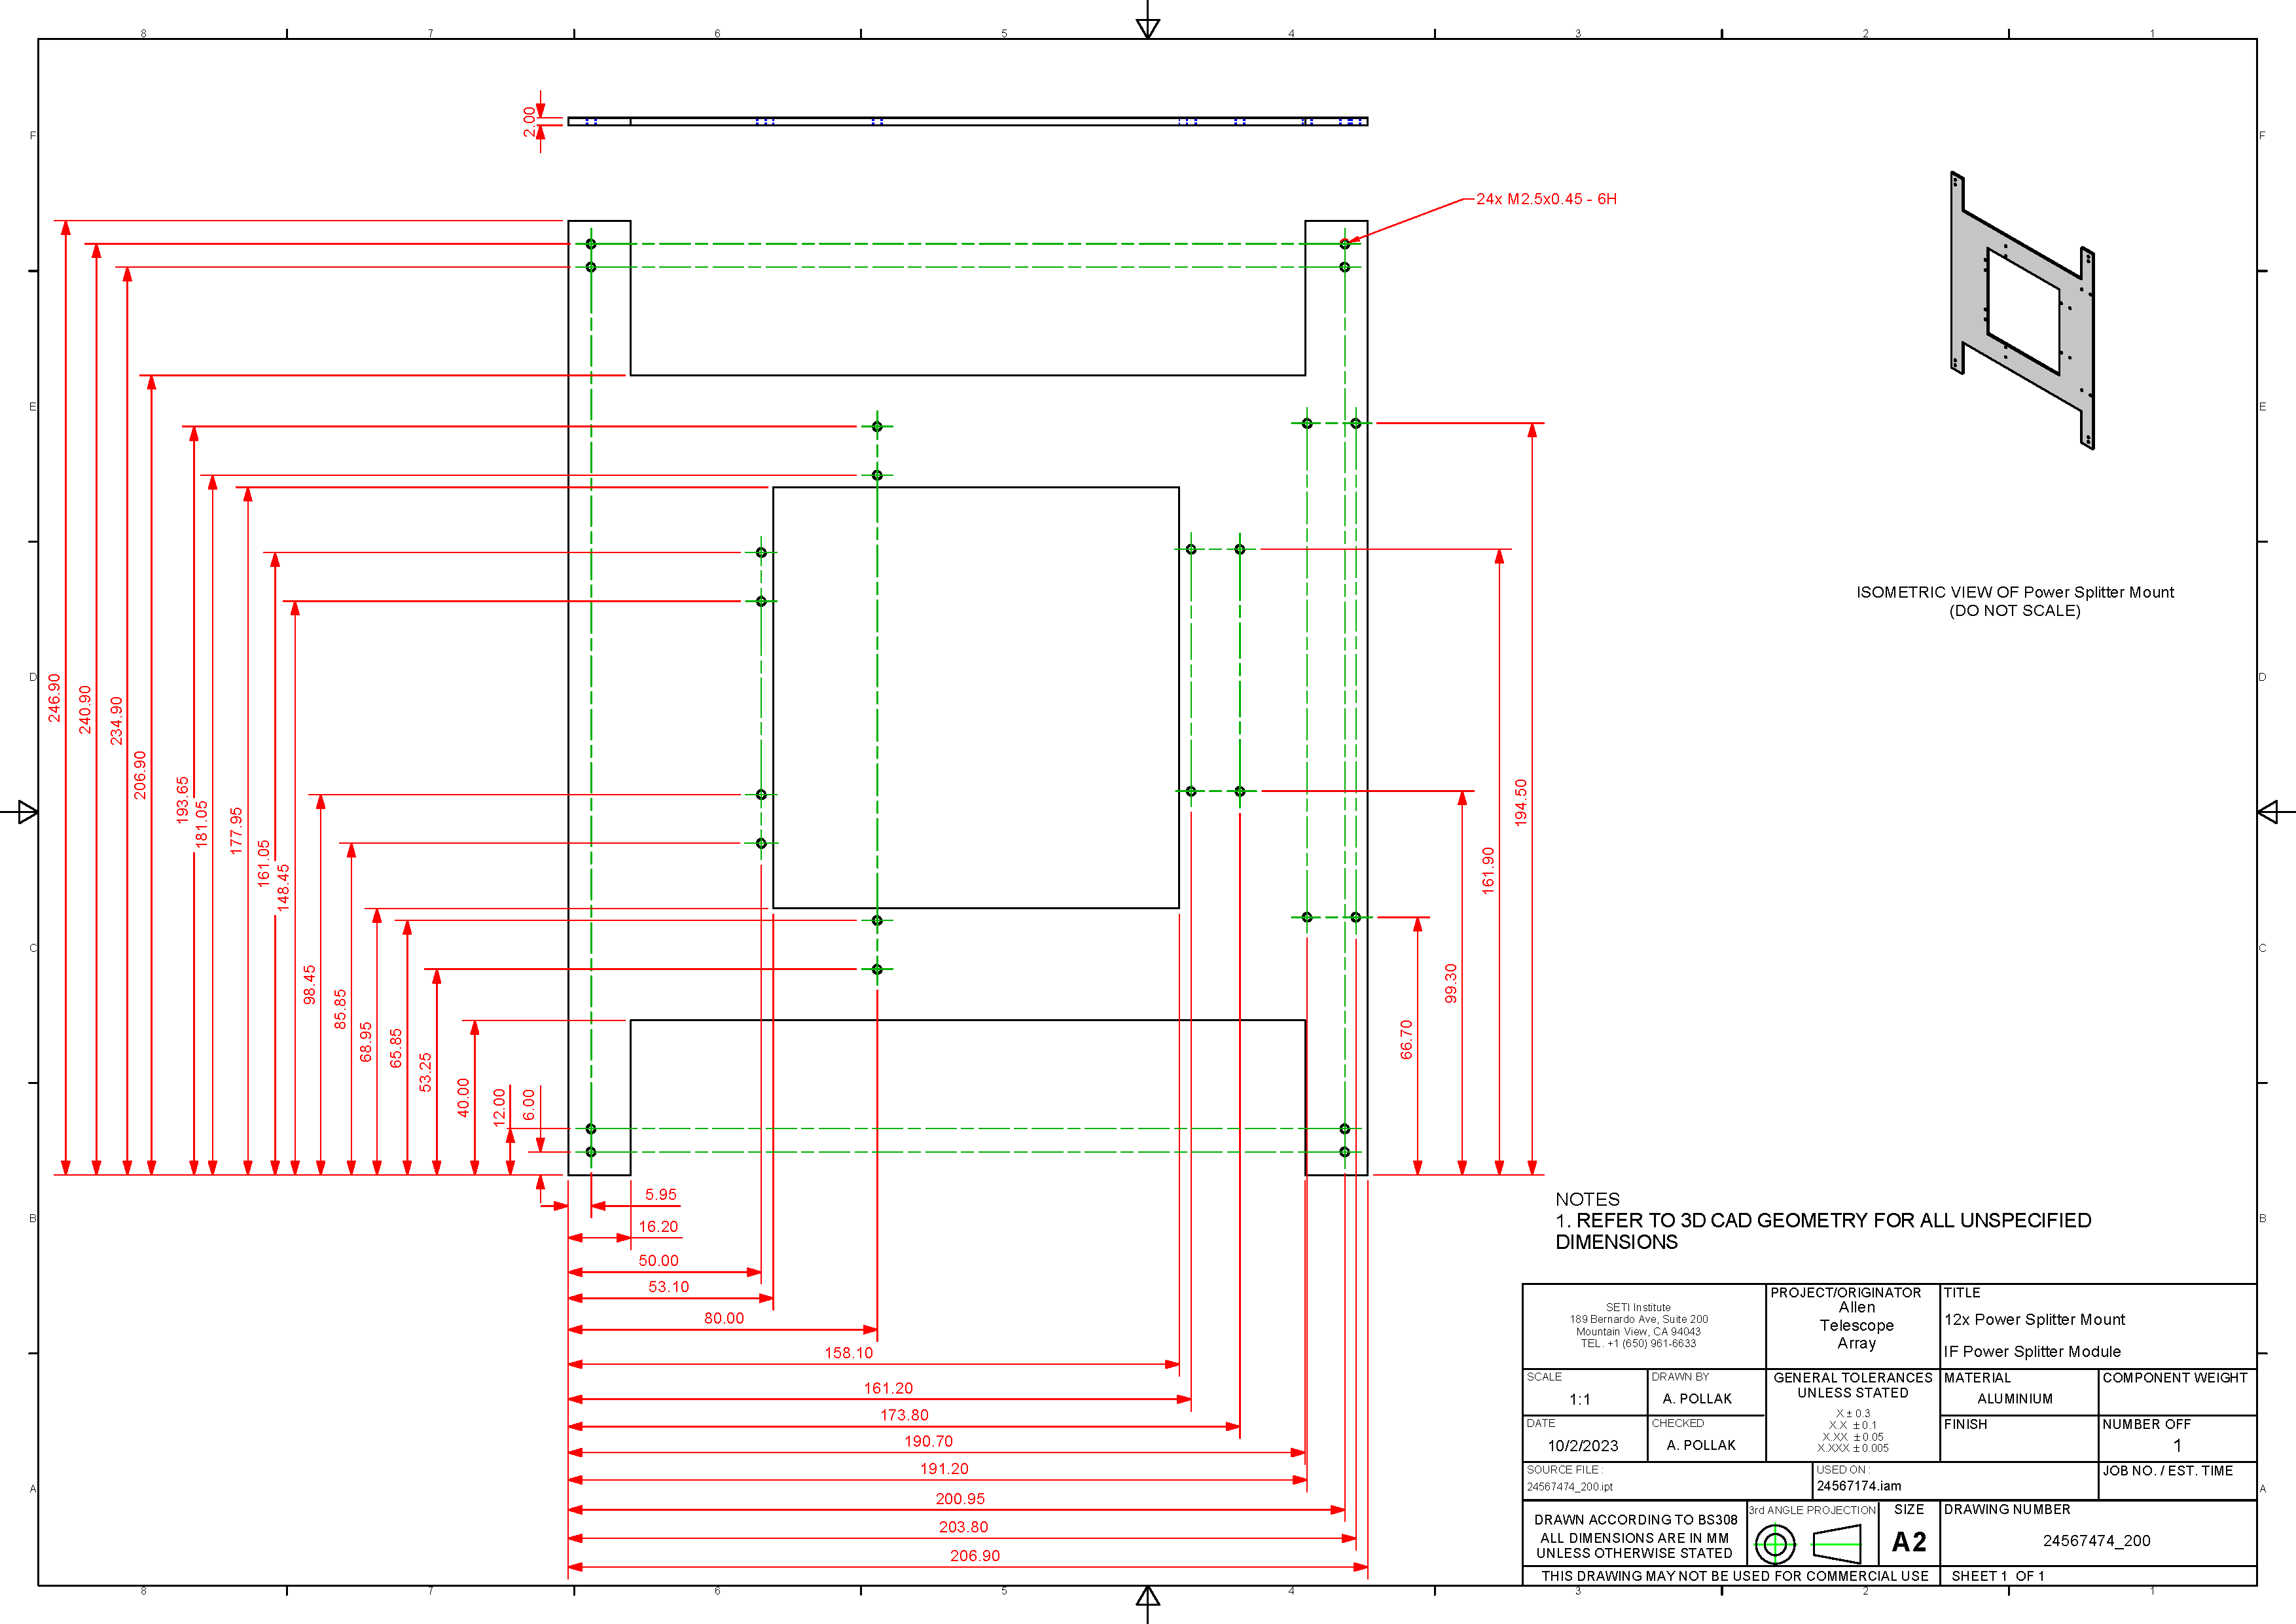
\includepdf[pages=-, landscape=true]{PDFs/24567474_200.pdf}
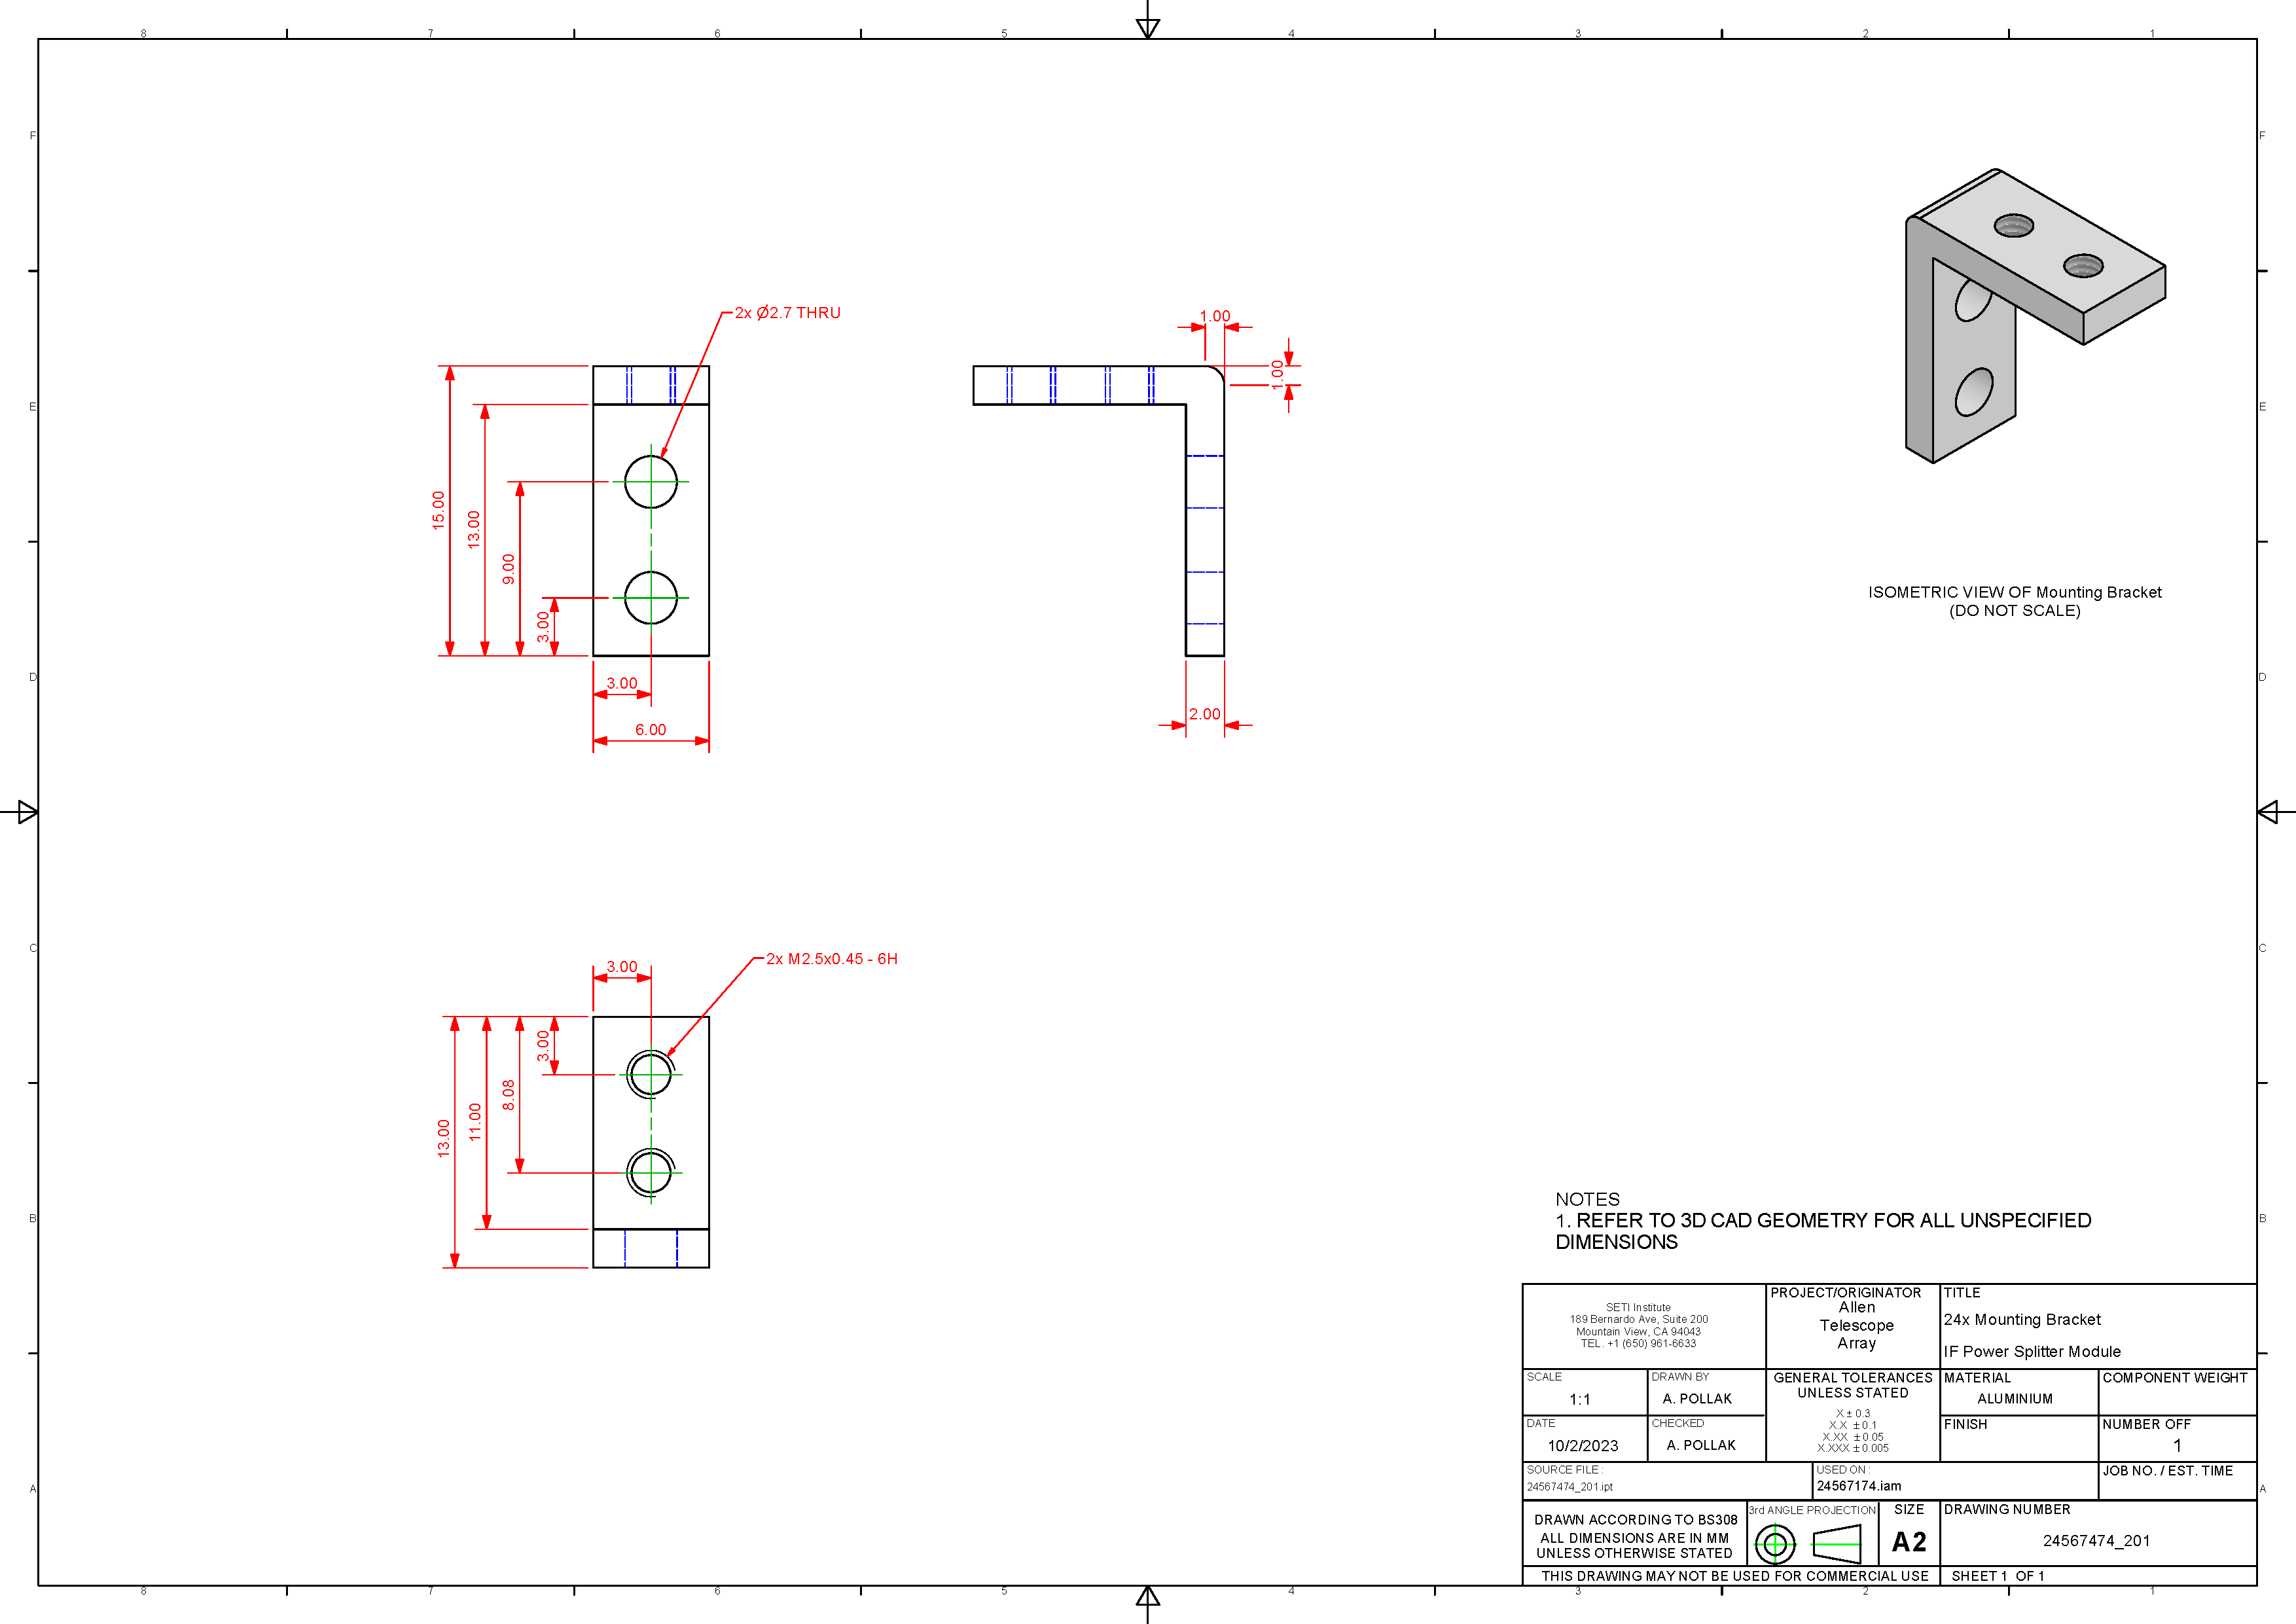
\includepdf[pages=-, landscape=true]{PDFs/24567474_201.pdf}
% ----------------------------------------------------------------


\end{landscape}

%
%\begin{figure}[H]
%\centering
%\includegraphics[width=1\linewidth]{<path>/picture.png}
%\caption{Caption}
%\label{fig:LABEL}
%\end{figure}
%

\end{document}
